\documentclass[12pt]{article}
\usepackage{amsmath,amssymb}
\usepackage{geometry}
\geometry{margin=1in}
\usepackage{tikz}
\usetikzlibrary{arrows.meta,calc,decorations.pathmorphing}

\begin{document}

\begin{center}
\Large \textbf{Advanced Integrated Physics Problem Set}\\
\large Ultra-Hard Level (Elite JEE Advanced / IAT)
\end{center}

\bigskip

%%%%%%%%%%%%%%%%%%%%%%%%%%%%%%%%%%%%%%%%%%%%%%%%%%%%%%%%%%%%

\textbf{Q1.}

A small bead of mass $m$ carrying charge $q$ is constrained to move without friction on a rigid circular ring of radius $R$. The ring rotates with constant angular speed $\omega$ about a vertical diameter passing through its center while a uniform magnetic field $B\hat z$ fills the region. The gravitational field acts vertically downward and the bead is allowed to attain steady equilibrium in the rotating frame.

Taking into account Coriolis effects, Lorentz force, and constraint reactions, determine the equilibrium angular position measured from the lowest point of the ring.

% Q1 Corrected Diagram
\begin{center}
\begin{tikzpicture}[scale=1]

% Ring
\draw (0,0) circle (2);

% Vertical rotation axis
\draw[->,thick] (0,-2.8)--(0,2.8) node[above] {$\omega$};

% Vertical magnetic field (into page cross-section symbol replaced by vertical arrow)
\draw[->,thick] (3,-1)--(3,1) node[above] {$B\hat z$};

% Bead at angle theta measured from lowest point
\coordinate (C) at (0,0);
\coordinate (Lowest) at (0,-2);
\coordinate (Bead) at ({2*sin(40)},{-2*cos(40)});

\fill (Bead) circle (2pt);

% Radius
\draw[dashed] (C)--(Bead);

% Vertical reference line
\draw[dashed] (C)--(Lowest);

% Angle mark
\draw (0,-0.8) arc (-90:-50:0.8);
\node at (-0.5,-1.1) {$\theta$};

\end{tikzpicture}
\end{center}

\begin{enumerate}
\item[(A)] $\displaystyle \frac{mg}{R(m\omega^2+qB\omega)}$
\item[(B)] $\displaystyle \frac{mg}{R(m\omega^2-qB\omega)}$
\item[(C)] $\displaystyle \frac{mg}{R(m\omega^2+2qB\omega)}$
\item[(D)] $\displaystyle \frac{mg}{R(m\omega^2-2qB\omega)}$
\end{enumerate}

%%%%%%%%%%%%%%%%%%%%%%%%%%%%%%%%%%%%%%%%%%%%%%%%%%%%%%%%%%%%

\textbf{Q2.}

A particle of mass $m$ slides in a narrow radial groove cut on a horizontal disc rotating with constant angular velocity $\omega$. The particle is attached to the center by a light spring of stiffness $k$ and natural length negligible compared to equilibrium radius. Small radial perturbations are given while ensuring no tangential motion relative to groove walls.

Accounting for centrifugal stiffening and Coriolis coupling, determine the frequency of small oscillations about equilibrium.

\begin{enumerate}
\item[(A)] $\sqrt{\frac{k}{m}-\omega^2}$
\item[(B)] $\sqrt{\frac{k}{m}-2\omega^2}$
\item[(C)] $\sqrt{\frac{k}{m}-3\omega^2}$
\item[(D)] $\sqrt{\frac{k}{m}+\omega^2}$
\end{enumerate}

%%%%%%%%%%%%%%%%%%%%%%%%%%%%%%%%%%%%%%%%%%%%%%%%%%%%%%%%%%%%

\textbf{Q3.}

A charged bead of mass $m$ is constrained to move along a fixed smooth helix of radius $R$ and pitch $p$. The helix axis is vertical and a uniform magnetic field acts parallel to the axis while gravity acts downward. The bead is projected such that motion becomes steady along the helix with constant speed.

Using generalized coordinate along helix and effective potential formulation, determine the condition corresponding to minimum effective potential.

% Q3 Corrected Helix
\begin{center}
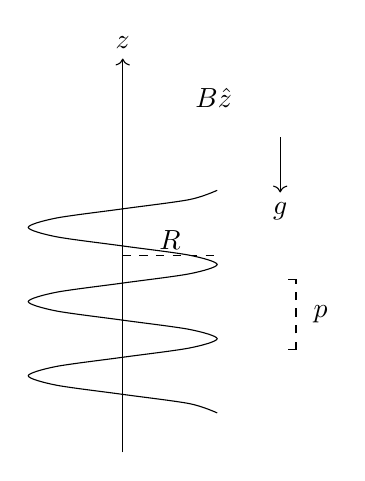
\begin{tikzpicture}[scale=1]

% Axis
\draw[->] (0,-2.5)--(0,2.5) node[above] {$z$};

% Helix (projected)
\draw[domain=0:6*pi,smooth,variable=\t]
plot ({1.2*cos(\t r)}, {0.15*\t -2});

% Magnetic field
\node[right] at (0.8,2) {$B\hat z$};

% Gravity
\draw[->] (2,1.5)--(2,0.8) node[below] {$g$};

% Radius marker
\draw[dashed] (0,0)--(1.2,0);

\node at (0.6,0.2) {$R$};

% Pitch marker (vertical separation between turns)
\draw[dashed] (2.2,-1.2)--(2.2,-0.3);
\draw[dashed] (2.1,-1.2)--(2.3,-1.2);
\draw[dashed] (2.1,-0.3)--(2.3,-0.3);
\node[right] at (2.3,-0.75) {$p$};

\end{tikzpicture}
\end{center}

\begin{enumerate}
\item[(A)] $\displaystyle \frac{mgp}{2\pi R qB}$
\item[(B)] $\displaystyle \frac{mgp}{qBR}$
\item[(C)] $\displaystyle \frac{2\pi mgR}{qBp}$
\item[(D)] $\displaystyle \frac{mg}{qB}$
\end{enumerate}

%%%%%%%%%%%%%%%%%%%%%%%%%%%%%%%%%%%%%%%%%%%%%%%%%%%%%%%%%%%%

\textbf{Q4.}

A light rigid rod of length $L$ carries charges $+q$ and $-q$ at its ends and is pivoted about its midpoint. The system is placed in a uniform electric field $E$ lying in the plane of motion and a uniform magnetic field perpendicular to the plane. The rod is slightly displaced from stable equilibrium and released with small angular velocity.

Considering induced magnetic torque due to motion of charges and restoring electrostatic torque, determine the angular frequency of small oscillations.

% Q4 Diagram
\begin{center}
\begin{tikzpicture}[scale=1]
\draw[thick] (-2,0)--(2,0);
\fill (0,0) circle (2pt);
\node at (-2.3,0) {$+q$};
\node at (2.3,0) {$-q$};
\draw[->] (0,-1.5)--(0,-2.5) node[below] {$E$};
\node at (0,1.5) {$B \ \otimes$};
\end{tikzpicture}
\end{center}

\begin{enumerate}
\item[(A)] $\sqrt{\frac{qEL}{I}}$
\item[(B)] $\sqrt{\frac{qEL}{I} - \frac{q^2B^2L^2}{4I^2}}$
\item[(C)] $\sqrt{\frac{qEL}{2I}}$
\item[(D)] $\sqrt{\frac{qEL}{2I} - \frac{q^2B^2L^2}{4I^2}}$
\end{enumerate}

%%%%%%%%%%%%%%%%%%%%%%%%%%%%%%%%%%%%%%%%%%%%%%%%%%%%%%%%%%%%

\textbf{Q5.}

Two particles of masses $m$ and $2m$ are connected by a light spring of stiffness $k$ and are constrained to move radially on a smooth horizontal rotating platform of angular speed $\omega$. The center of mass is held fixed by a frictionless radial guide while the spring remains along the radial direction.

Derive the normal mode frequency corresponding to symmetric oscillations taking into account centrifugal corrections.
% Q5 Diagram
\begin{center}
\begin{tikzpicture}[scale=1]
\draw (0,0) circle (2);
\fill (-1,0) circle (2pt) node[below] {$m$};
\fill (1,0) circle (2pt) node[below] {$2m$};
\draw[thick] (-1,0)--(1,0);
\draw[->] (0,-2.5)--(0,-3.5) node[below] {$\omega$};
\end{tikzpicture}
\end{center}

\begin{enumerate}
\item[(A)] $\sqrt{\frac{3k}{2m}-\omega^2}$
\item[(B)] $\sqrt{\frac{3k}{m}-\omega^2}$
\item[(C)] $\sqrt{\frac{3k}{2m}-2\omega^2}$
\item[(D)] $\sqrt{\frac{3k}{m}-2\omega^2}$
\end{enumerate}

%%%%%%%%%%%%%%%%%%%%%%%%%%%%%%%%%%%%%%%%%%%%%%%%%%%%%%%%%%%%

\textbf{Q6.}

A conducting circular loop of radius $R$, mass $m$, and resistance $R_0$ slides down a rough incline of angle $\alpha$ without slipping. A uniform magnetic field perpendicular to the plane of the incline exists everywhere. As the loop accelerates, motional emf induces current leading to magnetic braking torque.

After sufficient time the loop reaches steady motion. Determine the terminal speed considering both translational and rotational dynamics.

% Q6 Corrected Diagram
\begin{center}
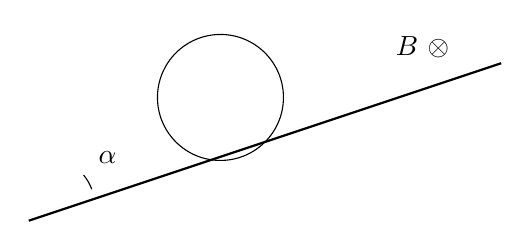
\begin{tikzpicture}[scale=1]

% Incline
\draw[thick] (-3,-1)--(3,1);

% Angle marker
\draw (-2.2,-0.6) arc (20:40:0.6);
\node at (-2,-0.2) {$\alpha$};

% Loop touching plane
\draw (-0.5657,0.5657) circle (0.8);
\draw[dashed] (-0.6,-0.2)--(0.6,0.2);

% Magnetic field into page
\node at (2,1.2) {$B \ \otimes$};

\end{tikzpicture}
\end{center}

\begin{enumerate}
\item[(A)] $\frac{mgR_0\sin\alpha}{2B^2R^2}$
\item[(B)] $\frac{mgR_0\sin\alpha}{B^2R^2}$
\item[(C)] $\frac{2mgR_0\sin\alpha}{B^2R^2}$
\item[(D)] $\frac{mgR_0\sin\alpha}{4B^2R^2}$
\end{enumerate}

%%%%%%%%%%%%%%%%%%%%%%%%%%%%%%%%%%%%%%%%%%%%%%%%%%%%%%%%%%%%

\textbf{Q7.}

A satellite of mass $m$ revolves around a planet of mass $M$ in a circular orbit of radius $r_0$. A small outward radial thrust proportional to inverse square distance acts continuously such that its magnitude is $ \epsilon GMm/r^2 $ where $ \epsilon \ll 1 $. Assume angular momentum adjusts adiabatically.

Determine the first-order correction to orbital radius maintaining circular motion.

\begin{enumerate}
\item[(A)] $r_0(1+\epsilon)$
\item[(B)] $r_0(1-\epsilon)$
\item[(C)] $r_0(1+2\epsilon)$
\item[(D)] $r_0(1-\frac{\epsilon}{2})$
\end{enumerate}

%%%%%%%%%%%%%%%%%%%%%%%%%%%%%%%%%%%%%%%%%%%%%%%%%%%%%%%%%%%%

\textbf{Q8.}

A parallel plate capacitor connected to an ideal battery maintains constant potential difference $V$. A dielectric slab of dielectric constant $\kappa$ is partially inserted between the plates and attached to a light spring of stiffness $k$. The slab can move freely without friction along insertion direction.

After equilibrium, the slab is displaced slightly and released. Using energy method including electrostatic work by battery, determine the frequency of small oscillations.

% Q8 Diagram
\begin{center}
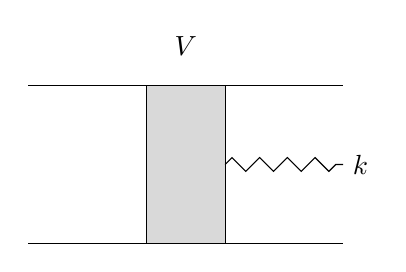
\begin{tikzpicture}[scale=1]
\draw (-2,1)--(2,1);
\draw (-2,-1)--(2,-1);
\draw[fill=gray!30] (-0.5,-1)--(0.5,-1)--(0.5,1)--(-0.5,1)--cycle;
\draw[decorate,decoration={zigzag}] (0.5,0)--(2,0);
\node[right] at (2,0) {$k$};
\node at (0,1.5) {$V$};
\end{tikzpicture}
\end{center}

\begin{enumerate}
\item[(A)] $\sqrt{\frac{\epsilon_0AV^2(\kappa-1)}{mkd^3}}$
\item[(B)] $\sqrt{\frac{\epsilon_0AV^2(\kappa-1)^2}{mkd^3}}$
\item[(C)] $\sqrt{\frac{\epsilon_0AV^2}{mkd^3}}$
\item[(D)] $\sqrt{\frac{\epsilon_0AV^2(\kappa+1)}{mkd^3}}$
\end{enumerate}

%%%%%%%%%%%%%%%%%%%%%%%%%%%%%%%%%%%%%%%%%%%%%%%%%%%%%%%%%%%%

\textbf{Q9.}

A particle slides without friction on a cycloidal track whose cusp is at the lowest point. The entire track rotates with constant angular velocity $\omega$ about a vertical axis through the cusp. Small oscillations are performed about the lowest point.

Using expansion of effective potential near equilibrium and including centrifugal pseudo potential, determine oscillation frequency.

% Q9 Corrected Cycloid
\begin{center}
\begin{tikzpicture}[scale=1]

% Cycloid (shifted so cusp at origin and lowest)
\draw[domain=0:6.28,smooth,variable=\t]
plot ({\t - sin(\t)}, {-(1 - cos(\t))});

% Vertical rotation axis
\draw[->] (0,0)--(0,-2.5) node[below] {$\omega$};

\end{tikzpicture}
\end{center}

\begin{enumerate}
\item[(A)] $\sqrt{\frac{g}{4a}-\omega^2}$
\item[(B)] $\sqrt{\frac{g}{4a}-2\omega^2}$
\item[(C)] $\sqrt{\frac{g}{4a}+\omega^2}$
\item[(D)] $\sqrt{\frac{g}{4a}-3\omega^2}$
\end{enumerate}

%%%%%%%%%%%%%%%%%%%%%%%%%%%%%%%%%%%%%%%%%%%%%%%%%%%%%%%%%%%%

\textbf{Q10.}

Two identical pendulums each of length $l$ carry equal charges $q$ and are suspended from the same support so that their equilibrium separation is small compared to length. The system is placed in a uniform horizontal magnetic field perpendicular to plane of oscillation. Small coupled oscillations occur about equilibrium.

Determine the corrected natural frequency including electrostatic coupling while identifying whether magnetic field contributes at first order.

% Q10 Diagram
\begin{center}
\begin{tikzpicture}[scale=1]
\draw (-1,2)--(-0.5,0);
\draw (1,2)--(0.5,0);
\fill (-0.5,0) circle (2pt);
\fill (0.5,0) circle (2pt);
\node at (-0.5,-0.3) {$q$};
\node at (0.5,-0.3) {$q$};
\draw[->] (-2.2,2.3)--(-1.2,2.3) node[right] {$B$};
\end{tikzpicture}
\end{center}

\begin{enumerate}
\item[(A)] $\sqrt{\frac{g}{l}+\frac{kq^2}{ml^3}}$
\item[(B)] $\sqrt{\frac{g}{l}-\frac{kq^2}{ml^3}}$
\item[(C)] $\sqrt{\frac{g}{l}+\frac{2kq^2}{ml^3}}$
\item[(D)] $\sqrt{\frac{g}{l}-\frac{2kq^2}{ml^3}}$
\end{enumerate}

%%%%%%%%%%%%%%%%%%%%%%%%%%%%%%%%%%%%%%%%%%%%%%%%%%%%%%%%%%%%

\textbf{Q11.}

A particle moves under central potential  
\[
U(r)=\frac12 kr^2-\frac{\alpha}{r}
\]
and executes circular motion at radius $r_0$. Small radial perturbations are introduced while angular momentum remains conserved.

Using effective potential expansion up to second order, determine radial oscillation frequency.

\begin{enumerate}
\item[(A)] $\sqrt{\frac{k}{m}+\frac{3\alpha}{mr_0^3}}$
\item[(B)] $\sqrt{\frac{3k}{m}+\frac{\alpha}{mr_0^3}}$
\item[(C)] $\sqrt{\frac{3k}{m}-\frac{\alpha}{mr_0^3}}$
\item[(D)] $\sqrt{\frac{k}{m}-\frac{3\alpha}{mr_0^3}}$
\end{enumerate}

%%%%%%%%%%%%%%%%%%%%%%%%%%%%%%%%%%%%%%%%%%%%%%%%%%%%%%%%%%%%

\textbf{Q12.}

A conducting rod of length $L$ slides without friction on parallel rails inclined at angle $\theta$. The rails are connected to a capacitor of capacitance $C$ and a uniform magnetic field is perpendicular to the plane of rails. The system starts from rest with capacitor uncharged.

Determine the maximum speed attained by the rod using energy conservation including electrostatic energy stored.

% Q12 Corrected Diagram
\begin{center}
\begin{tikzpicture}[scale=1]

% Rails
\draw (-2,-1)--(2,1);
\draw (-2,-2)--(2,0);

% Sliding rod
\draw (-0.5,-1.5)--(1.5,0.5);

% Capacitor connected to rails
\draw (2,1)--(3,1);
\draw (2,0)--(3,0);
\draw (3,1)--(3,0);
\draw (3.4,1)--(3.4,0);
\draw (3.4,1)--(4,1);
\draw (3.4,0)--(4,0);
\node[right] at (4,0.5) {$C$};

% Magnetic field
\node at (2.2,1.5) {$B \ \otimes$};

% Angle
\node at (-2,-2.3) {$\theta$};

\end{tikzpicture}
\end{center}

\begin{enumerate}
\item[(A)] $\sqrt{\frac{mgL\sin\theta}{B^2C}}$
\item[(B)] $\sqrt{\frac{2mgL\sin\theta}{B^2C}}$
\item[(C)] $\frac{mgL\sin\theta}{B^2C}$
\item[(D)] $\frac{2mgL\sin\theta}{B^2C}$
\end{enumerate}

%%%%%%%%%%%%%%%%%%%%%%%%%%%%%%%%%%%%%%%%%%%%%%%%%%%%%%%%%%%%

\textbf{Q13.}

A thin ring rolls without slipping inside a vertical circular hoop which itself rotates about its vertical diameter with constant angular speed $\omega$. Consider motion near the topmost point of hoop and include rolling constraint properly.

Determine condition on $\omega$ for stable equilibrium at the top.

% Q13 Corrected Diagram
\begin{center}
\begin{tikzpicture}[scale=1]

% Outer hoop
\draw (0,0) circle (2);

% Inner rolling ring touching inside at top
\draw (0,1.6) circle (0.4);

% Rotation axis
\draw[->] (0,-2.5)--(0,-3.5) node[below] {$\omega$};

\end{tikzpicture}
\end{center}

\begin{enumerate}
\item[(A)] $\omega^2>\frac{g}{R}$
\item[(B)] $\omega^2>\frac{2g}{R}$
\item[(C)] $\omega^2>\frac{3g}{R}$
\item[(D)] $\omega^2>\frac{4g}{R}$
\end{enumerate}

%%%%%%%%%%%%%%%%%%%%%%%%%%%%%%%%%%%%%%%%%%%%%%%%%%%%%%%%%%%%

\textbf{Q14.}

An LC circuit contains a parallel plate capacitor whose dielectric slab is attached to a block of mass $m$ connected to a spring of stiffness $k$. The electrical oscillations and mechanical motion are weakly coupled through capacitance variation with displacement. Small oscillations occur about equilibrium when circuit is charged to voltage $V$.

Determine the lower normal mode frequency of the coupled system.

% Q14 Diagram
\begin{center}
\begin{tikzpicture}[scale=1]
\draw (-3,0)--(-1,0);
\draw (-1,1)--(-1,-1);
\draw (1,1)--(1,-1);
\draw (1,0)--(3,0);
\draw[decorate,decoration={zigzag}] (3,0)--(4.5,0);
\node[right] at (4.5,0) {$k$};
\node at (0,1.5) {$C$};
\node at (-2,0.5) {$L$};
\draw (-3,0)--(-3,-1.5)--(4.5,-1.5)--(4.5,0);
\end{tikzpicture}
\end{center}

\begin{enumerate}
\item[(A)] $\sqrt{\frac{k}{m}}$
\item[(B)] $\sqrt{\frac{k}{m}-\frac{V^2}{mLCd^2}}$
\item[(C)] $\sqrt{\frac{k}{m}+\frac{V^2}{mLCd^2}}$
\item[(D)] $\sqrt{\frac{k}{m}-\frac{2V^2}{mLCd^2}}$
\end{enumerate}

%%%%%%%%%%%%%%%%%%%%%%%%%%%%%%%%%%%%%%%%%%%%%%%%%%%%%%%%%%%%

\textbf{Q15.}

A particle moves in a rotating frame with angular velocity $\omega$ where effective potential is  
\[
U=-\frac{GMm}{r}+\frac12 m\omega^2 r^2.
\]
Small radial perturbations are introduced about equilibrium circular orbit.

Determine equilibrium radius and comment on stability condition.

\begin{enumerate}
\item[(A)] $\left(\frac{GM}{\omega^2}\right)^{1/3}$
\item[(B)] $\left(\frac{2GM}{\omega^2}\right)^{1/3}$
\item[(C)] $\left(\frac{GM}{2\omega^2}\right)^{1/3}$
\item[(D)] $\left(\frac{3GM}{\omega^2}\right)^{1/3}$
\end{enumerate}

%%%%%%%%%%%%%%%%%%%%%%%%%%%%%%%%%%%%%%%%%%%%%%%%%%%%%%%%%%%%

\end{document}